% ─── Slide: Digital Quantisation — pipeline + histograms ─────────────────────
\begin{frame}[shrink=25]{Digital Quantisation}

  \vspace{-0.3em}
  \begin{center}
  \begin{tikzpicture}[
      every node/.style={font=\scriptsize},
      dq/.style={draw=mybluedark, rounded corners=2pt, fill=myblue!22,
                 minimum width=1.6cm, minimum height=0.68cm, align=center},
      tile/.style={draw=mybluedark, rounded corners=2pt, fill=mybluedark!15,
                   text=mybluedark, minimum width=2.0cm, minimum height=0.88cm,
                   align=center},
      adc/.style={draw, rounded corners=2pt, fill=myorange!30,
                  minimum width=1.3cm, minimum height=0.68cm, align=center},
      outbox/.style={draw, rounded corners=2pt, fill=mygreen!20,
                  minimum width=0.9cm, minimum height=0.68cm, align=center},
      arr/.style={-{Latex[length=1.3mm]}, thick},
      histbox/.style={draw=mygray!55, thin, rounded corners=2pt,
                      fill=white, inner sep=1pt},
      link/.style={dashed, mygray!60, line width=0.4pt}
    ]

    % ─── Pipeline ─────────────────────────────────────────────────────────
    \node (w)  at (0,   0.8) {$w$};
    \node[dq]  (qw) at (1.5,  0.8) {Digital\\quantiser};
    \node (wb) at (3.0,  0.8) {$\hat w$};

    \node (x)  at (0,  -0.8) {$x$};
    \node[dq]  (qx) at (1.5, -0.8) {Digital\\quantiser};
    \node (xb) at (3.0, -0.8) {$\hat x$};

    \draw[arr] (w)--(qw);  \draw[arr] (qw)--(wb);
    \draw[arr] (x)--(qx);  \draw[arr] (qx)--(xb);

    \node[tile] (T) at (4.9, 0) {Analog IMC tile\\$y{=}\langle\hat w,\hat x\rangle$};
    \draw[arr] (wb) -- (T.north west);
    \draw[arr] (xb) -- (T.south west);

    \node (y)  at (6.5, 0) {$y$};
    \draw[arr] (T) -- node[above=-1pt, font=\tiny]{$y\!\in\!\mathbb{Z}$} (y);

    \node[adc] (A) at (7.7, 0) {ADC\\$\lfloor y/\delta\rfloor$};
    \draw[arr] (y)--(A);

    \node[outbox] (yb) at (9.2, 0) {$\hat y$};
    \draw[arr] (A)--(yb);

    % ─── Histograms ───────────────────────────────────────────────────────
    \node[histbox] (hw)  at (0,   2.3) {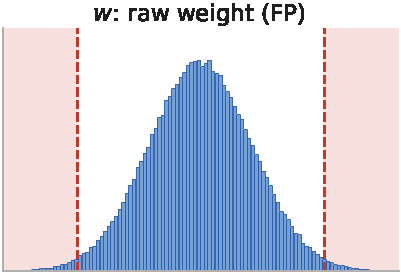
\includegraphics[width=2.2cm]{figs/dist_w.pdf}};
    \node[histbox] (hwb) at (3.0, 2.3) {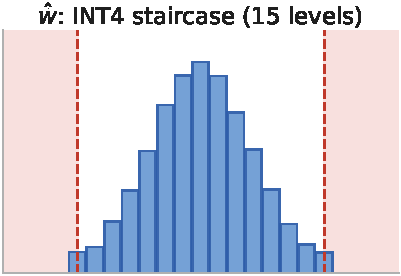
\includegraphics[width=2.2cm]{figs/dist_w_hat.pdf}};
    \draw[link] (hw.south)  -- (w.north);
    \draw[link] (hwb.south) -- (wb.north);

    \node[histbox] (hx)  at (0,  -2.3) {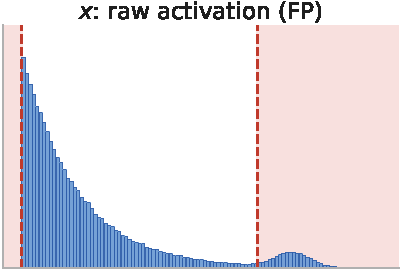
\includegraphics[width=2.2cm]{figs/dist_x.pdf}};
    \node[histbox] (hxb) at (3.0,-2.3) {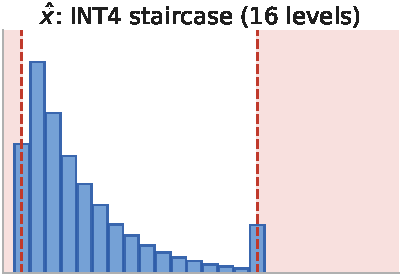
\includegraphics[width=2.2cm]{figs/dist_x_hat.pdf}};
    \draw[link] (hx.north)  -- (x.south);
    \draw[link] (hxb.north) -- (xb.south);

    \node[histbox] (hy) at (6.3, 2.3) {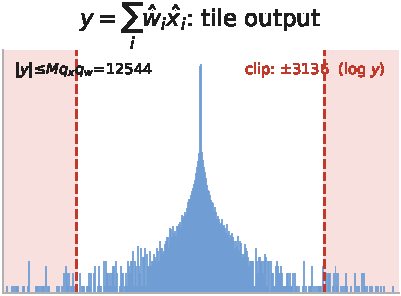
\includegraphics[width=2.2cm]{figs/dist_y.pdf}};
    \draw[link] (hy.south) -- (y.north);

    % ─── Blue zone: quantisation + integer MVM ────────────────────────────
    \begin{pgfonlayer}{background}
      \node[inner sep=9pt, draw=mybluedark, line width=1.5pt,
            rounded corners=7pt, fill=myblue!6,
            fit=(hw)(hwb)(hy)(hx)(hxb)(w)(qw)(wb)(x)(qx)(xb)(T)(y)] (Z1) {};
    \end{pgfonlayer}
    \node[anchor=north west, font=\scriptsize\bfseries, text=mybluedark,
          xshift=4pt, yshift=-4pt] at (Z1.north west)
      {Quantisation + integer MVM};

  \end{tikzpicture}
  \end{center}

  \vspace{-0.1em}
  {\footnotesize\centering
    \textbf{Quantise:}\enspace
    $\hat v = \mathrm{clip}\!\left(\lfloor v/s\rfloor,\,-q,\,q\right)$,\enspace
    $s={\max|v|}/{q}$,\enspace $q=2^{b-1}{-}1$
    \hspace{1.5em}
    \textbf{Dequantise:}\enspace $\tilde v = s\cdot\hat v$\par}

  \note{Зум в синий прямоугольник. Квантизация — округление с масштабом, деквантизация — умножение обратно. Гистограммы показывают что происходит с распределением весов и активаций до и после.}

\end{frame}
